\documentclass[10pt]{jarticle}
\usepackage{ascmac}
\usepackage[dvipdfmx]{graphicx}
\usepackage{enumerate}
\usepackage{amsmath,amssymb}
\usepackage{url}
\usepackage{enumitem}
\usepackage{listings}
\usepackage{comment}
\usepackage[hang,small,bf]{caption}
\usepackage[subrefformat=parens]{subcaption}
\renewcommand{\lstlistingname}{source}
\lstset{language=sh,%
        basicstyle=\footnotesize,%
	commentstyle=\textit,%
	classoffset=1,%
	keywordstyle=\bfseries,%
	frame=shadowbox,framesep=4pt,%
	showstringspaces=false%,
	numbers=left,stepnumber=1,numberstyle=\footnotesize,%
	numbersep=1zw,%
	lineskip=-0.5ex,%
	xleftmargin=2zw%
	}%

\newdimen\paperwidth \newdimen\paperheight
\def\A4size{\paperwidth=210mm \paperheight=297mm}
\def\centered{%
  \oddsidemargin=\paperwidth
  \advance\oddsidemargin-\textwidth
  \oddsidemargin=0.5\oddsidemargin
  \advance\oddsidemargin-1in
  \evensidemargin-\oddsidemargin}
%
\textwidth 160mm
\textheight 230mm
\topmargin 0mm
\headheight 0mm
\footskip 0mm
\A4size\centered

\title{\framebox{\hspace{4zw}モーター レポート2%
                 \hspace{4zw}}}
\author{神野 友哉 \\
        2022311042  \\
        愛知県立大学 情報科学部 情報科学科 \\}
\date{2024年1月14日}


\begin{document}
\maketitle
\tableofcontents
\clearpage


\section{課題 6}
%
同定実験\ 1\ で得られた結果に対して、(25)式への当てはまり具合を確認すると、何らかの誤差を観察できるはずである。
どの程度の誤差か説明し、その誤差が生じた物理的要因を多角的に検討して洞察せよ。
%

\subsection{目的}
%
モーターに入力する電圧に対して必ずしもタコメータの出力電圧が比例しない原因を調査する。
%

\subsection{考察}
%
この同定実験において、ソースコード\ref{id}を使用する。
その際、$U_{min}=1.0$、$U_{max}=1.7$と入力した。
図\ref{fig:kadai6}は、そうした近似曲線の当てはめによって得られた結果である。

\begin{figure}[htbp]
	\begin{center}
		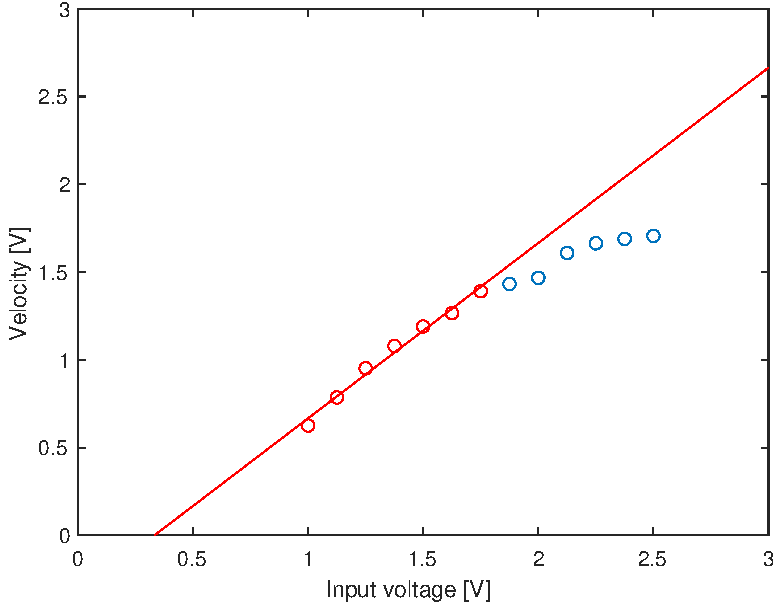
\includegraphics[width=100mm]{wk3/DJ1-crop.pdf}
	\end{center}
	\caption{入力電圧と出力の関係}
	\label{fig:kadai6}
\end{figure}

図\ref{fig:kadai6}を観察すると、横軸\ Input\ voltage\ 1.7V\ 未満は近似曲線に概ね従っていることと、
\ 1.7V\ 以降、近似曲線よりも低い値を取っていることが解かる。
つまり、入力電圧に対して、出力が完全には比例していないことを示しているのである。
その原因を考察する。まず、モデルでは、モーターに入力する電圧を$v_{a}$とし、タコメータの出力電圧を$v_{o}$、ゲインを$K$とすると、
\begin{equation}
		v_{o}=Kv_{a} \label{eq:kadai6}
\end{equation}
の関係式で表せるはずである。しかし、式(\ref{eq:kadai6})のように完全に比例するというのはモデルの仮定であり、
実際には、導線の抵抗や湿度、気温、モーターのコイル巻き数、ブラシや整流子の摩擦
等々\cite{kadai6}、モデルが影響力を無視している概念が多くある。そのため、このような結果が得られたと考えられる。

\lstinputlisting[caption=velo\_id\_gain.m, label=id]{./velo_id_gain.m}

%

\subsection{結論}
%
モデルはあくまでモデルであり、ある程度の求められる成果を得られればよい。そのため、現実の物理現象を完全に網羅したモデルは存在しえないのだろう。
%


\section{課題 7}
%
$p_{1}=p_{2}$のもと、望みの極を実軸上で様々に変化させると、応答はどのように変化するか、
実験結果をもとに、極と応答の間にどんな関係性があるか考察せよ。
%

\subsection{目的}
%
極の複素数の実数部が持つ、ゲインや応答に対する意味合いを調査する。
%

\subsection{考察}
%
以降の極指定法の課題でソースコード\ref{pi}を使用する。また、同定実験\ 2\ で得られたパラメータ$K、T、u_{offset}$の値は、
それぞれ、$0.816865、0.480000、0.047711$である。これらも、以降の極指定法で利用する。
極入力は$p_{1}=p_{2}=  1,  2, -1, -2$として、それぞれ応答を確かめた結果が図\ref{fig:kadai7}である。
\begin{figure}[htbp]
	\begin{center}
		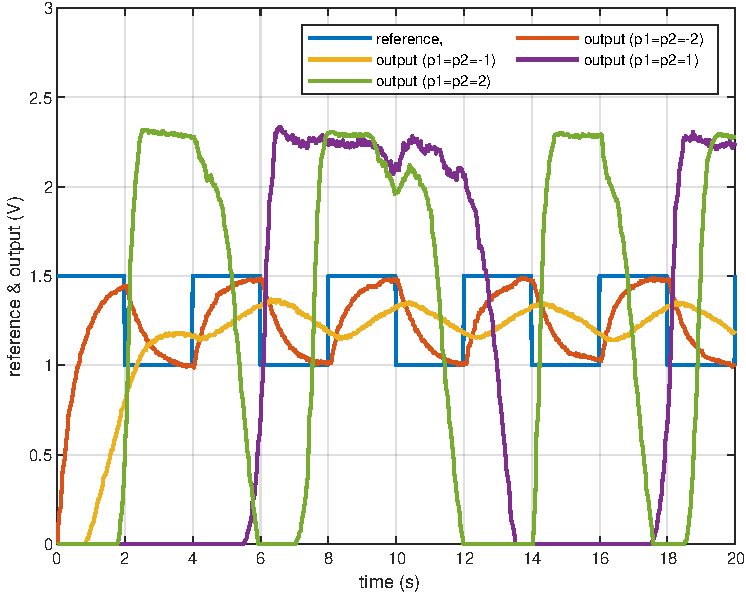
\includegraphics[width=100mm]{wk3/p1p2-equal-0-crop.pdf}
	\end{center}
	\caption{実数部のみ調整}
	\label{fig:kadai7}
\end{figure}
$p_{1}=p_{2}$の符号が負である場合(-1, -2)、目標値に沿うように近づいていることが解かる。
図をよく観察すると、極の符号が正の方向で増加すると、横軸区間\ times\ 2-6\ のように、急上昇するタイミングが
早くなっていると判り、逆に極の符号が府の方向で増加すると、同様に横軸区間\ times\ 2-6\ のように、目標値に近づくのが早いと判る。

\begin{eqnarray}
K_{P} &=& -\frac{(p_{1} + p_{2})T + 1}{K} \label{eq:kadai7no1}\\
K_{I} &=& \frac{p_{1}p_{2}T}{K} \label{eq:kadai7no2}
\end{eqnarray}

これは、極と比例ゲインの関係式(\ref{eq:kadai7no1})と、極と積分ゲインの関係式(\ref{eq:kadai7no2})から
原因が考察できる。なぜなら、比例・積分両ゲインの符号は正である必要があり、
それを満たすような$p_{1}、p_{2}$の取り方の条件を確かめることが可能であることが理由である。
比例ゲインの場合は、式(\ref{eq:kadai7no1})の右辺$\geq 0$として$p_{1} + p_{2}$について解く。
\begin{eqnarray*}
	T > 0 かつ K > 0 とし \\
	-\frac{(p_{1} + p_{2})T + 1}{K} &\geq& 0 \\
	-\frac{1}{K} \leq 0 で両辺割り、不等式反転 \\
	(p_{1} + p_{2})T + 1 &\leq& 0 \\
	両辺から 1 を引き、T > 0 で両辺割る \\
	(p_{1} + p_{2}) &\leq& -\frac{1}{T} \\
	-\frac{1}{T} < 0 なので、 \\
	(p_{1} + p_{2}) &<& 0 
\end{eqnarray*}
また、積分ゲインの場合も、式(\ref{eq:kadai7no2})の右辺$\geq 0$として$p_{1}p_{2}$について解く。
\begin{eqnarray*}
	\frac{p_{1}p_{2}T}{K} &\geq& 0 \\
	\frac{T}{K} > 0 で両辺割り \\
	p_{1}p_{2} &\geq& 0
\end{eqnarray*}
以上をまとめた、
\begin{eqnarray*}
	(p_{1} + p_{2}) &<& 0 \label{eq:kadai7no3}\\
	p_{1}p_{2} &\geq& 0 \label{eq:kadai7no4}
\end{eqnarray*}
を同時に満たせる$p_{1}、p_{2}$の条件は、$p_{1} < 0 かつ p_{2} < 0$または$一方 < 0 でもう一方 = 0 $の場合である。
今回は$p_{1}=p_{2}$であるため、前者の条件のみ$p_{1}=p_{2}= -1, -2$の値で満たし、このような結果になったと言える。

\lstinputlisting[caption=velo\_pi\_mbd.m, label=pi]{./velo_pi_mbd.m}

%

\subsection{結論}
%
ゲイン調整の極指定法で極を選ぶ際に、極の複素数の実部の符号が負であることが好ましいと解かった。
%


\section{課題 8}
%
$p_{1}$、$p_{2}$を共役な複素数としたとき、望みの極を虚軸と平行な方向に様々に変化させると、
応答はどのように変化するか、実験結果をもとに、極と応答の間にどんな関係性があるか考察せよ。
%

\subsection{目的}
%
極の複素数の虚数部が持つ、ゲインと応答に対する意味合いを調査する。
%

\subsection{考察}
%
$p_{1}= -2-a\times i, p_{2}=-2+a\times i$の$a$に$0.5、 1、2、3$を代入して、虚軸に平行に変化させ、応答の変化を観察する。
結果は図\ref{fig:kadai8}となった。
\begin{figure}[htbp]
	\begin{center}
		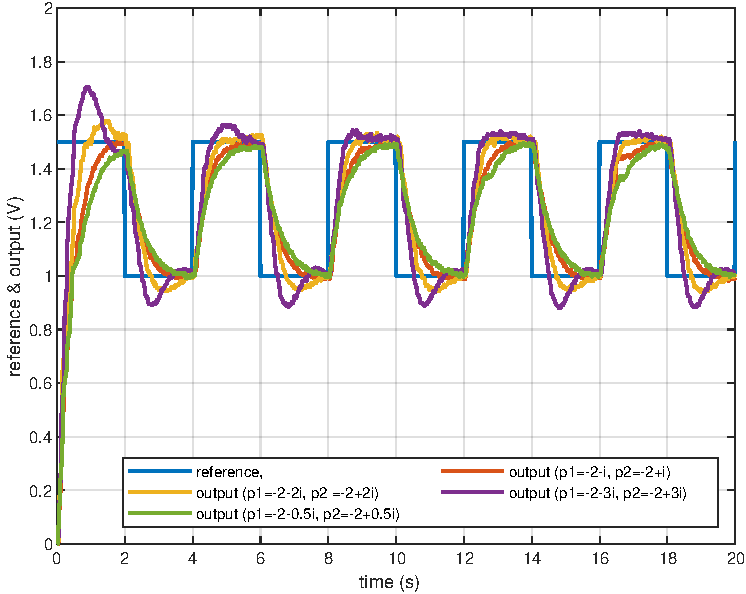
\includegraphics[width=100mm]{wk3/p1p2-image-crop.pdf}
	\end{center}
	\caption{虚数部のみ調整}
	\label{fig:kadai8}
\end{figure}
横軸\ time\ の区間\ 0-2\ や\ 12-14\ が判りやすいが、$a$に代入した値が大きい程、目標値に早く近づく傾向にあるのは明白である。
その原因をゲインと極の関係式の構造から考察する。
課題\ 7\ の$k_{P}$ゲインの式(\ref{eq:kadai7no1})は$p_{1} + p_{2}$、
$k_{I}$ゲインの式(\ref{eq:kadai7no2})は$p_{1}p_{2}$、つまり$p_{1}、p_{2}$の基本対称式の形を含む。
$p_{1}、p_{2}$が共役な複素数である場合に、$p_{1} + p_{2}$も$p_{1}p_{2}$も虚部が、$p_{1}、p_{2}$のそれぞれの虚部に関係なく\ 0\ となり消滅する。
しかし、$p_{1} + p_{2}$と$p_{1}p_{2}$のそれぞれの実部は、$p_{1}、p_{2}$の$実部 \times 2$と$実部^{2} + 虚部^{2}$である。
つまり、極の複素数の虚部のみを変化させた場合に、$k_{P}$ゲインには影響しないと考えられるが、$k_{I}$ゲインの大きさに影響すると考えられる。
そのため、極の虚部の値が増加するにつれて、$k_{I}$ゲインが大きくなり、出力の振動を抑制し、目標値に早く収束させる働きが強まったと考えられる。

%

\subsection{結論}
%
極の複素数が共役である場合、その虚部は$k_{I}$ゲインのみに影響し、実部は$k_{P}$ゲインと$k_{I}$ゲインに影響する。
具体的には、極の実部絶対値の増加により$k_{P}、k_{I}$両ゲインが増加し、虚部絶対値の増加は$k_{I}$ゲインのみ増加する。
%


\section{課題 9}
%
$PI$ゲインの設計問題に対して、モデルを用いないアプローチとモデルを用いるアプローチをとった、調整や設計における手間(時間的コスト)
や得られた結果といった観点から、\ 2\ つのアプローチを比較評価せよ。
%

\subsection{目的}
%
ゲイン調整を目的とする各アプローチの特徴を探求する。
%

\subsection{考察}
%
限界感度法というモデルを用いないアプローチの場合、掛けた時間は約\ 30\ 分で、一方、極指定法というモデルを用いるアプローチの場合は約\ 20\ 分であった。
それは、準備の時間等を全て含む上での経過時間であり、調整・設計において、モデルを用いるアプローチが時間効率の面で優れていること、
これこそ実際の実験で判明したことである。加えて、極指定法の極は、ゲインに虚数を含まない意図で共役な複素数であることや、課題\ 7\ と課題\ 8\ の結論を考慮すると、
人間にとって扱いやすい・都合がよいように設計されていると考えられ、極とゲインの関係式の作りにより、手間の観点からも効率的なゲイン調整が可能であると判明した。
しかし、得られた結果としては、極指定法によって調整されたゲインの出力が、限界感度法のそれよりも
目標値への収束が遅かったため、実機における$K_{P}$ゲインの適正値よりも低いと考えられるが、
先ほどの議論から微調整が容易であると考えられるため、大それた問題ではないのだろう。

%

\subsection{結論}
%
今回は、モデルを用いるゲイン調整アプローチに極指定法を用いたが、それは、モデルが実機にある程度、適合していることが絶対の前提条件であるため、
満たしていることを仮定して利用した。結果として、モデルを利用する極指定法がモデルを利用しない限界感度法と比較して、
時間・手間の観点で効率が良いと判断した。

%


\section{課題 10}
%
[自由]\ モデルを用いないアプローチで得たゲインを極として評価し、
極指定法で得た極と比較・議論せよ。
%

\subsection{目的}
%
モデルを用いないアプローチである限界感度法と、モデルを用いるアプローチである極指定法の応答の違いを考察する。
%

\subsection{考察}
%
モデルを用いないアプローチとして限界感度法を利用した。
限界感度法で得たゲインは$ K_{P}=11、K_{I}=74 $であった。
式(\ref{eq:kadai7no1})を$ p_{1} + p_{2} $について解く。
\begin{eqnarray*}
	K_{P} &=& -\frac{(p_{1} + p_{2})T + 1}{K} \\
	p_{1} + p_{2} &=& \frac{-K_{P}K - 1}{T} \\
	K_{P} = 11、K = 0.816865、T &=& 0.480000 より \\
	p_{1} + p_{2} &=& -20.803156 \\
	0 に近づける切り捨て \\
	&\fallingdotseq& -20 \\
\end{eqnarray*}
また、式(\ref{eq:kadai7no2})も$p_{1}p_{2}$について解く。
\begin{eqnarray*}
	K_{I} &=& \frac{p_{1}p_{2}T}{K} \\
	p_{1}p_{2} &=& \frac{K_{I}K}{T} \\
	K_{I} = 74、K = 0.816865、T &=& 0.480000 より \\
	p_{1}p_{2} &=& 125.933354 \\
	0 に近づける切り捨て \\
	&\fallingdotseq& 125 \\
\end{eqnarray*}
$ p_{1}、p_{2} $の基本対称式の形なので、二次方程式の解と係数の関係より、
\begin{eqnarray*}
	x^{2} - (p_{1} + p_{2})x + p_{1}p_{2} &=& 0 \\
	p_{1} + p_{2} = -20、p_{1}p_{2} &=& 125 より\\
	x^{2} + 20x + 125 &=& 0 \\
	解の公式より、\\
	x &=& -10 \pm 5i
\end{eqnarray*}
よって、限界感度法のゲインを極として評価した場合、極は$ p_{1} = -10 - 5i、p_{2} = -10 + 5i $となる。
一方で、極指定法で得た極は$ p_{1} = -7 - 5i、p_{2} = -7 + 5i $である。
それらを極指定法プログラムに入力した結果は、図\ref{fig:kadai10}となった。
\begin{figure}[htbp]
	\begin{center}
		
\includegraphics[width=100mm]{./wk3/kadai10-crop.pdf}
	\end{center}
	\caption{モデルを用いないアプローチによる極入力}
	\label{fig:kadai10}
\end{figure}
横軸\ time\ の区間\ 0-2\ をよく観察すると、極指定法の極での応答は、限界感度法のゲインの極での応答より目標値への収束が遅いことが判る。
これは、課題\ 9\ の考察で言及したことである。一方で、横軸\ time\ の区間\ 2-4\ 、\ 6-8\ 、\ 10-12\ 、\ 14-16\ 、\ 18-20\ から、
限界感度法では、目標値の電圧が下がる局面で、大きく振動していることも判る。
この結果が得られた原因を考察する。入力した極の複素数を比較すると、
限界感度法の実部の絶対値の方が大きいことが解かり、課題\ 8\ の結論により、
限界感度法の方が$k_{P}$、$k_{I}$両ゲインが大きいことが判る。そのため、
$実部 \times 2$を計算式に含む$k_{P}$の増加は収束を高速にしたが、$実部^{2}$を含む$K_{I}$ゲインが過度に増加したため、
限界感度法の応答が振動気味になっていると考えられる。

%

\subsection{結論}
%
課題\ 9\ の結論と似た内容になるのは避けられず、極指定法が時間・手間の観点で効率が良いと考えられる。
その具体的に判断した根拠をこの課題\ 10\ にて言及したに過ぎなかった。

%

\begin{thebibliography}{5}
  \bibitem{kadai2}
    今井: "電源回路の比例制御と積分制御", Wave Technology. 2022, \\
    \url{https://www.wti.jp/contents/blog/blog220628.htm}, (参照 2024-1-16).
	\bibitem{kadai6}
	  モーターメンテナンス.com: "モーターのよくあるトラブルとその対策方法は？", モーターメンテナンス.com. 2023, \\
		\url{https://industrial-motor-maintenance.com/column/troubleshooting/505/}, (参照 2024-1-16).
\end{thebibliography}
\end{document}
